\documentclass[12pt,a4paper]{article}
\usepackage[utf8]{inputenc}
\usepackage[spanish]{babel}
\usepackage{amsmath}
\usepackage{amsfonts}
\usepackage{amssymb}
\usepackage{graphicx}
\usepackage{geometry}
\usepackage{fancyhdr}
\usepackage{xcolor}
\usepackage{listings}
\usepackage{enumitem}

% Configuración de página
\geometry{margin=2.5cm}
\pagestyle{fancy}
\fancyhf{}
\rhead{Universidad Nacional del Altiplano - FINESI}
\lhead{Optimización}
\cfoot{\thepage}

% Configuración para código Python
\lstset{
    language=Python,
    basicstyle=\ttfamily\small,
    backgroundcolor=\color{gray!10},
    keywordstyle=\color{blue},
    commentstyle=\color{green!60!black},
    stringstyle=\color{red},
    showstringspaces=false,
    breaklines=true,
    frame=single,
    numbers=left,
    numberstyle=\tiny\color{gray}
}

\begin{document}

\begin{center}
\textbf{\Large Evaluación: Unidad II}\\
\vspace{0.5cm}
\textbf{Apellidos y Nombres:} Kenny Leonel Ccora Quispe
\end{center}

\vspace{1cm}

\section*{1. ¿Cuáles son las principales diferencias entre la optimización de funciones convexas y no convexas, y cómo influyen en la elección de métodos?}

Aquí las principales diferencias:

\subsection*{Funciones Convexas:}
\begin{itemize}[leftmargin=1.5cm]
    \item \textbf{Característica principal:} Cualquier mínimo local es también mínimo global
    \item \textbf{Ventajas:} Garantía de convergencia al óptimo global
    \item \textbf{Métodos efectivos:} Método de Newton, BFGS, métodos de punto interior
    \item \textbf{Aplicación en ML:} SVM, regresión lineal con regularización
\end{itemize}

\subsection*{Funciones No Convexas:}
\begin{itemize}[leftmargin=1.5cm]
    \item \textbf{Problema principal:} Múltiples mínimos locales
    \item \textbf{Desafíos:} Riesgo de quedar atrapados en soluciones subóptimas
    \item \textbf{Métodos necesarios:} Algoritmos evolutivos, PSO, algoritmos genéticos
    \item \textbf{Estrategias:} Múltiples inicializaciones, métodos estocásticos
\end{itemize}

\section*{2. ¿Cuándo resulta más efectivo usar variantes del descenso de gradiente y cuáles son los factores clave en su selección?}

Los criterios de optimalidad permiten determinar si una solución obtenida por un algoritmo es efectivamente óptima (ya sea local o global). En métodos de optimización, su aplicación depende del tipo de problema:

\subsection*{SGD básico:}
\begin{itemize}[leftmargin=1.5cm]
    \item \textbf{Uso efectivo:} Datasets grandes
    \item \textbf{Ventaja:} Menor costo computacional por iteración
    \item \textbf{Desventaja:} Convergencia ruidosa
\end{itemize}

\subsection*{SGD con Momentum:}
\begin{itemize}[leftmargin=1.5cm]
    \item \textbf{Uso efectivo:} Superficies con barrancos o mal condicionamiento
    \item \textbf{Ventaja:} Acelera convergencia, reduce oscilaciones
\end{itemize}

\subsection*{Algoritmos adaptativos (Adam, RMSprop, AdaGrad):}
\begin{itemize}[leftmargin=1.5cm]
    \item \textbf{Uso efectivo:} Mayoría de problemas de ML
    \item \textbf{Ventaja:} Ajuste automático del learning rate por parámetro
\end{itemize}

\subsection*{Factores clave de selección:}
\begin{itemize}[leftmargin=1.5cm]
    \item Tamaño del dataset
    \item Recursos computacionales disponibles
    \item Naturaleza de la función objetivo
    \item Necesidad de convergencia estable vs velocidad
\end{itemize}

\section*{3. ¿Cómo se aplican los criterios de optimalidad en un método de optimización?}

Los criterios de optimalidad permiten saber si una solución alcanzada por un algoritmo es suficientemente buena (óptima). Su aplicación varía según el tipo de problema, pero en términos generales se sigue este enfoque:

\subsection*{Sin restricciones:}
\begin{itemize}[leftmargin=1.5cm]
    \item \textbf{Condición necesaria:} $\nabla f(x^*) = 0$
    \item \textbf{Condición suficiente:} Hessiano positivo definido
    \item \textbf{Implementación:} Criterio de parada $\|\nabla f(x)\| < \epsilon$
\end{itemize}

\subsection*{Con restricciones de igualdad:}
\begin{itemize}[leftmargin=1.5cm]
    \item \textbf{Método:} Multiplicadores de Lagrange
    \item \textbf{Condiciones:} $\nabla L(x^*,\lambda^*) = 0$
\end{itemize}

\subsection*{Con restricciones de desigualdad:}
\begin{itemize}[leftmargin=1.5cm]
    \item \textbf{Condiciones KKT:} Gradiente del Lagrangiano = 0
    \item \textbf{Holguras complementarias:} $\lambda_i g_i(x^*) = 0$
    \item \textbf{Factibilidad:} $g_i(x^*) \leq 0$, $\lambda_i \geq 0$
\end{itemize}

\section*{4. ¿De qué manera facilitan las herramientas de optimización automática (p.ej., Optuna) la búsqueda de configuraciones óptimas en aprendizaje automático?}

Optuna y otras bibliotecas de optimización automática simplifican la tarea de encontrar hiperparámetros óptimos en modelos de machine learning, algo que manualmente puede ser lento y poco efectivo. Aquí cómo se hace:

\subsection*{Automatización inteligente:}
\begin{itemize}[leftmargin=1.5cm]
    \item \textbf{Algoritmos:} TPE (Tree-structured Parzen Estimator)
    \item \textbf{Aprendizaje:} Usa evaluaciones anteriores para proponer mejores configuraciones
    \item \textbf{Eficiencia:} Pruning automático elimina trials no prometedores
\end{itemize}

\subsection*{Beneficios prácticos:}
\begin{itemize}[leftmargin=1.5cm]
    \item \textbf{Paralelización:} Optimización distribuida
    \item \textbf{Integración:} Compatible con frameworks de ML (scikit-learn, TensorFlow)
    \item \textbf{Ahorro de tiempo:} Evita búsqueda manual exhaustiva
\end{itemize}

\section*{5. ¿Cómo influye la selección de estrategias de regularización en el desempeño y la generalización de un modelo?}

La regularización controla la complejidad del modelo para evitar que se ajuste demasiado a los datos de entrenamiento (overfitting). Aquí más detalles:

\subsection*{L1 (Lasso):}
\begin{itemize}[leftmargin=1.5cm]
    \item \textbf{Efecto:} Selección de características (sparsity)
    \item \textbf{Uso:} Cuando queremos pocas características relevantes
    \item \textbf{Impacto:} Reduce overfitting eliminando características irrelevantes
\end{itemize}

\subsection*{L2 (Ridge):}
\begin{itemize}[leftmargin=1.5cm]
    \item \textbf{Efecto:} Reduce magnitud de pesos sin eliminarlos
    \item \textbf{Uso:} Cuando todas las características son importantes
    \item \textbf{Impacto:} Mejora generalización suavizando el modelo
\end{itemize}

\subsection*{Elastic Net:}
\begin{itemize}[leftmargin=1.5cm]
    \item \textbf{Combinación:} L1 + L2
    \item \textbf{Uso:} Grupos de características correlacionadas
\end{itemize}

\subsection*{Impacto en desempeño:}
\begin{itemize}[leftmargin=1.5cm]
    \item \textbf{Bias-variance tradeoff:} Aumenta sesgo, reduce varianza
    \item \textbf{Generalización:} Mejora rendimiento en datos no vistos
    \item \textbf{Selección $\lambda$:} Validación cruzada para parámetro óptimo
\end{itemize}

\section*{6. ¿Cómo se pueden integrar rutinas de validación y corrección de código en Optuna para mejorar la calidad y eficacia del proceso de optimización de hiperparámetros?}

Incorporar rutinas de validación y corrección dentro del proceso de optimización con Optuna permite asegurar que cada prueba sea confiable, interpretable y reproducible. Aquí más detalles:

\subsection*{Rutinas de validación:}
\begin{itemize}[leftmargin=1.5cm]
    \item \textbf{Cross-validation:} Dentro de la función objetivo
    \item \textbf{Pruning:} \texttt{trial.report()} y \texttt{trial.should\_prune()}
    \item \textbf{Early stopping:} Basado en métricas de validación
\end{itemize}

\subsection*{Corrección y monitoreo:}
\begin{itemize}[leftmargin=1.5cm]
    \item \textbf{Logging:} Registro automático de todos los trials
    \item \textbf{Callbacks:} Guardar mejores modelos automáticamente
    \item \textbf{Manejo de errores:} Try-catch para trials fallidos
    \item \textbf{Visualización:} Optuna-dashboard para monitoreo en tiempo real
\end{itemize}

\section*{7. ¿Cómo podemos utilizar las métricas provistas por scikit-learn para evaluar un modelo de clasificación, y qué información adicional brindan además de la exactitud? Completa y Responde:}

Scikit-learn ofrece varias métricas que permiten evaluar modelos de clasificación con más profundidad que solo la exactitud (accuracy). Estas métricas revelan cómo se comporta el modelo frente a distintas clases, desequilibrios y errores.

\begin{figure}[h]
    \centering
    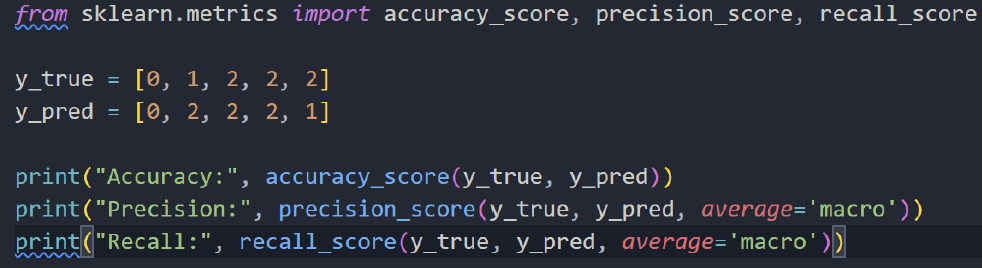
\includegraphics[width=0.8\textwidth]{codigo.png}
    \caption{Ejemplo de uso de métricas en scikit-learn}
    \label{fig:codigo}
\end{figure}

\textbf{Resultado:}
\begin{itemize}[leftmargin=1.5cm]
    \item Accuracy: 0.6
    \item Precision: 0.5555555555555555
    \item Recall: 0.5555555555555555
\end{itemize}

\subsection*{Información adicional:}

\subsubsection*{Precision:}
\begin{itemize}[leftmargin=1.5cm]
    \item \textbf{Mide:} De las predicciones positivas, cuántas fueron correctas
    \item \textbf{Fórmula:} TP / (TP + FP)
    \item \textbf{Importante:} Cuando falsos positivos son costosos
\end{itemize}

\subsubsection*{Recall:}
\begin{itemize}[leftmargin=1.5cm]
    \item \textbf{Mide:} De los casos positivos reales, cuántos fueron detectados
    \item \textbf{Fórmula:} TP / (TP + FN)
    \item \textbf{Importante:} Cuando falsos negativos son costosos
\end{itemize}

\subsection*{Ventajas sobre accuracy:}
\begin{itemize}[leftmargin=1.5cm]
    \item \textbf{Clases desbalanceadas:} Accuracy puede ser engañosa
    \item \textbf{Análisis por clase:} Identifica qué clases se predicen mal
    \item \textbf{F1-score:} Combina precision y recall en una métrica
    \item \textbf{Matriz de confusión:} Muestra errores específicos entre clases
\end{itemize}

\end{document}